\documentclass{article}
\usepackage{graphicx}

\title{chapter 3}
\author{Nurul Kamila (1184038) }
\date{November 2019}




\begin{document}

\maketitle
\section{Fungsi}
Fungsi adalah satu blok program yang terdiri dari nama fungsi, input variabel dan variabel kembalian.
contoh implementasi dari fungsi :
\begin{center}
    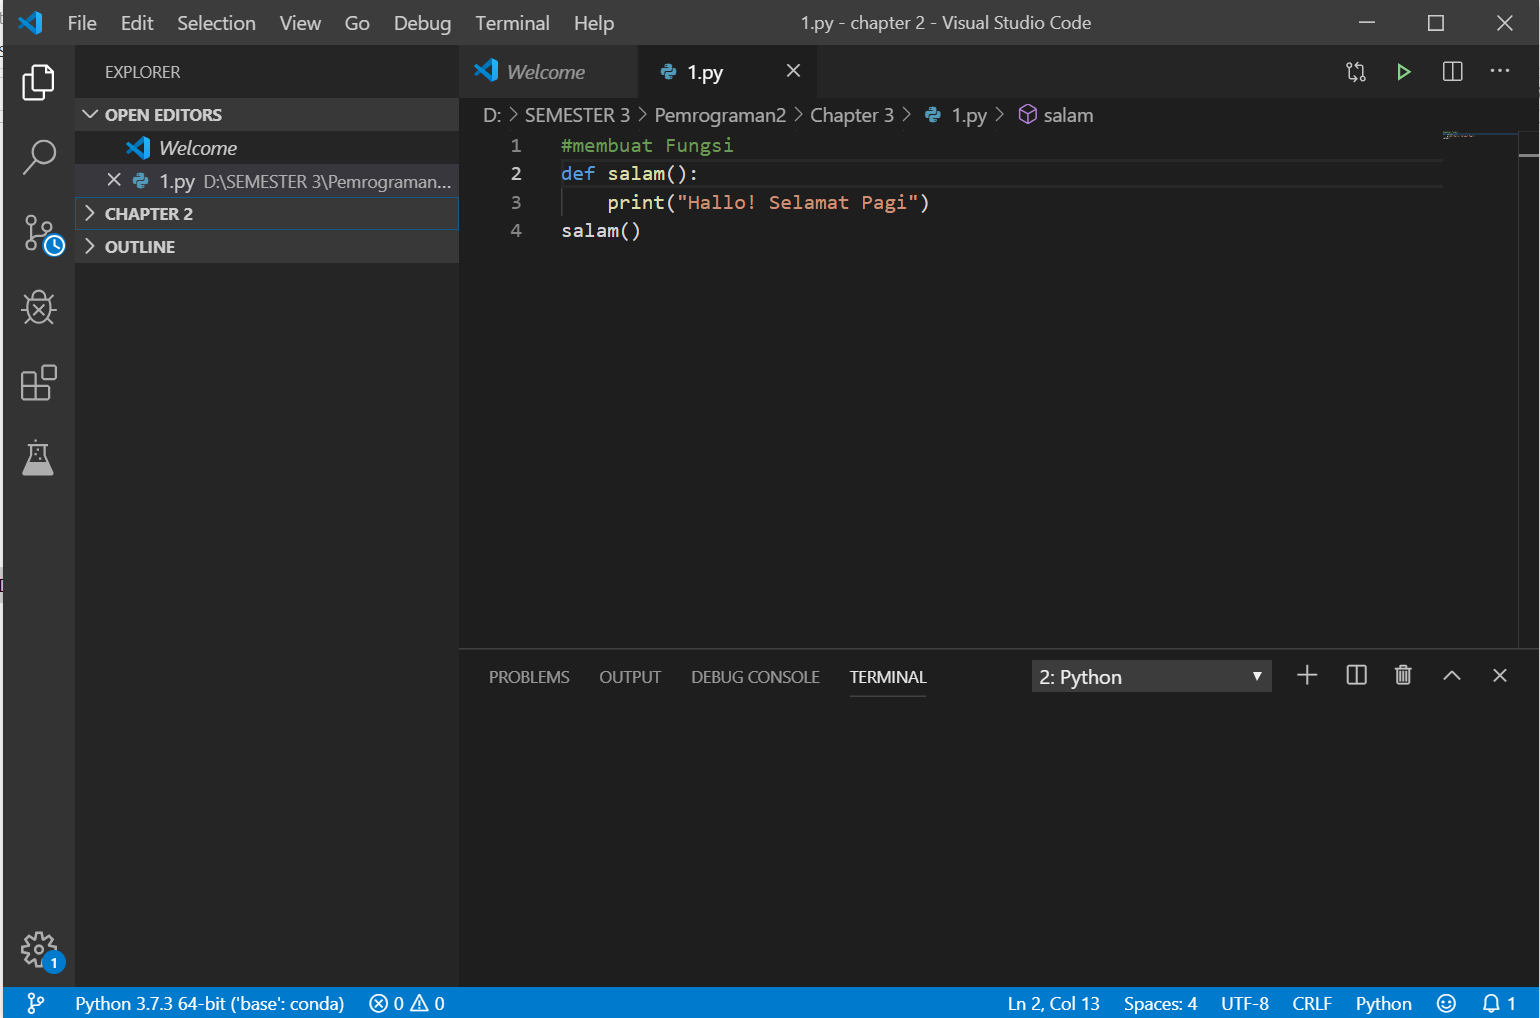
\includegraphics[width=.8\textwidth]{keterampilan/1.PNG}
\end{center}

\section{Package}
Package merupakan sekumpulan file atau modul yang terdapat sebuah fungsi yang dapat dijalankan. Cara pemanggilannya yaitu:
\begin{center}
    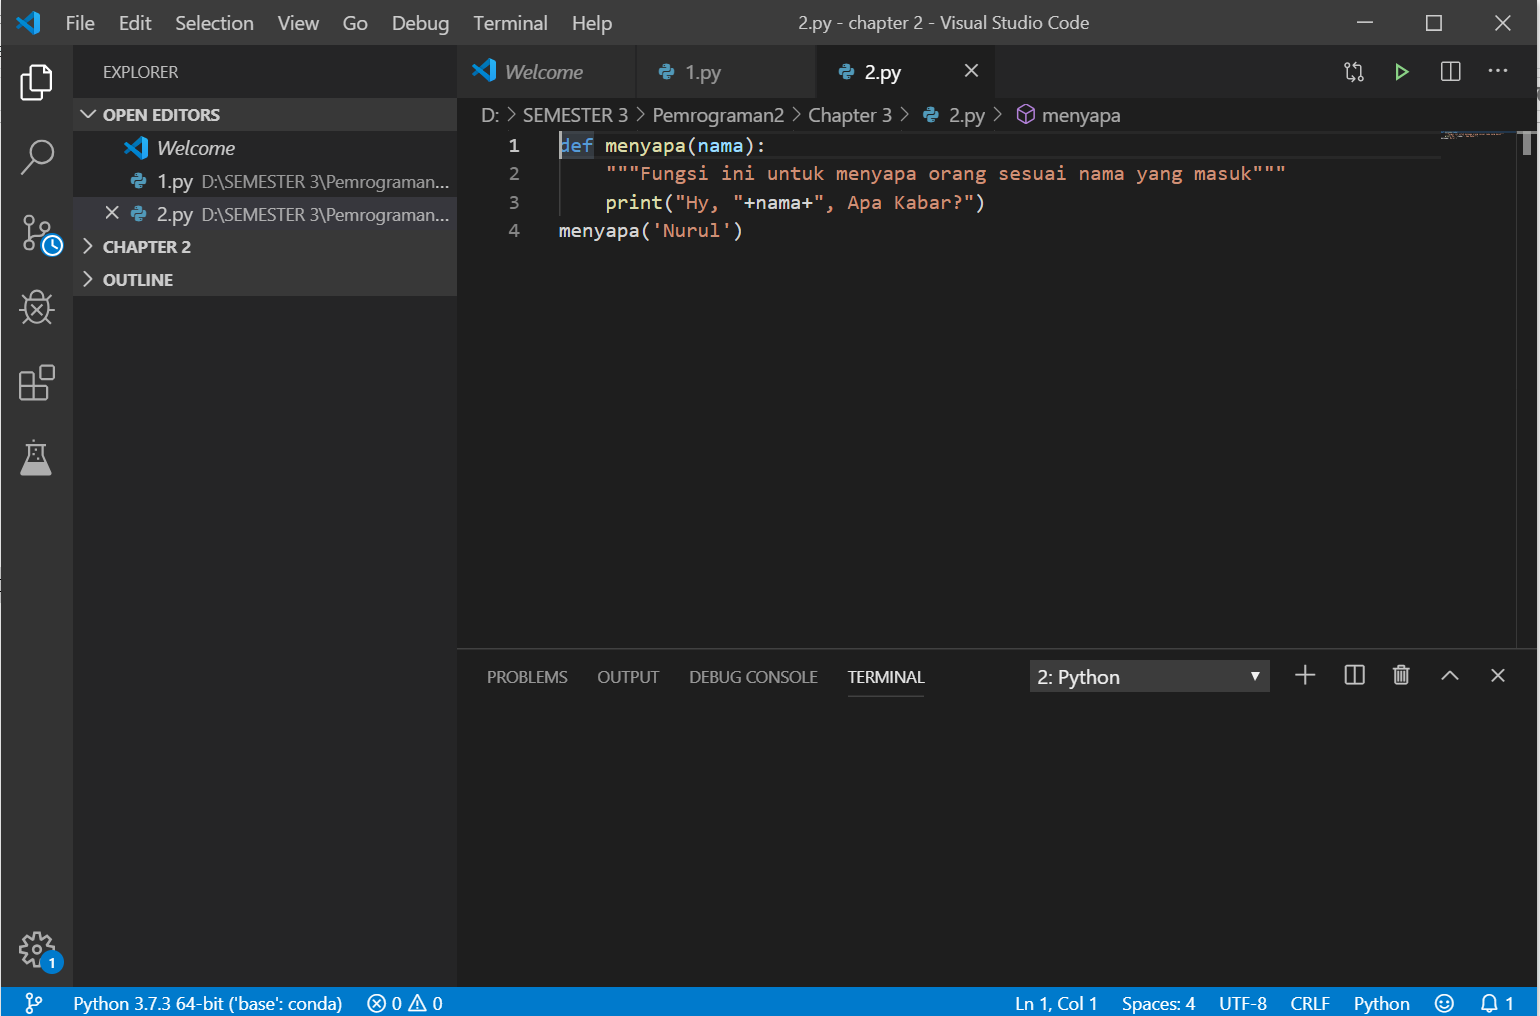
\includegraphics[width=.8\textwidth]{keterampilan/2.PNG}
\end{center}

\section{Class}
Class merupakan blueprint dari sebuah object.
\begin{center}
    \includegraphics[width=.8\textwidth]{keterampilan/3.PNG}
\end{center}

\section{Object}
Object merupakan bagian dari program yang berada dalam sebuah class.
\begin{center}
    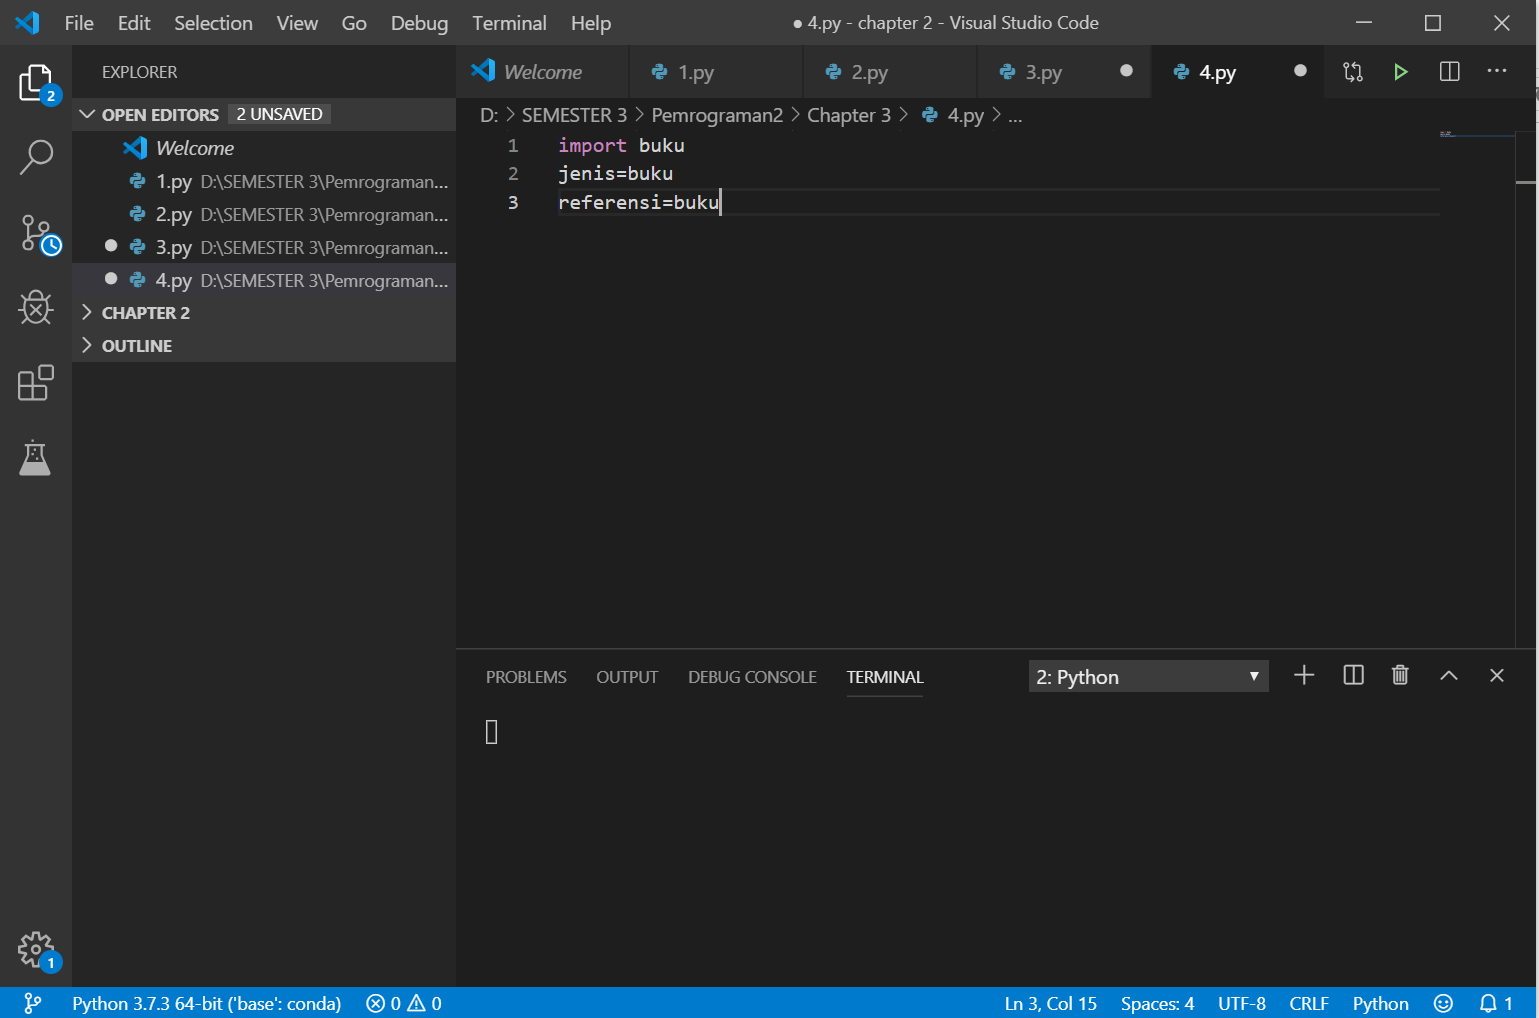
\includegraphics[width=.8\textwidth]{keterampilan/4.PNG}
\end{center}

\subsection{Atribute}
Atribute merupakan bagian yang dimiliki oleh sebuah class.
\begin{center}
    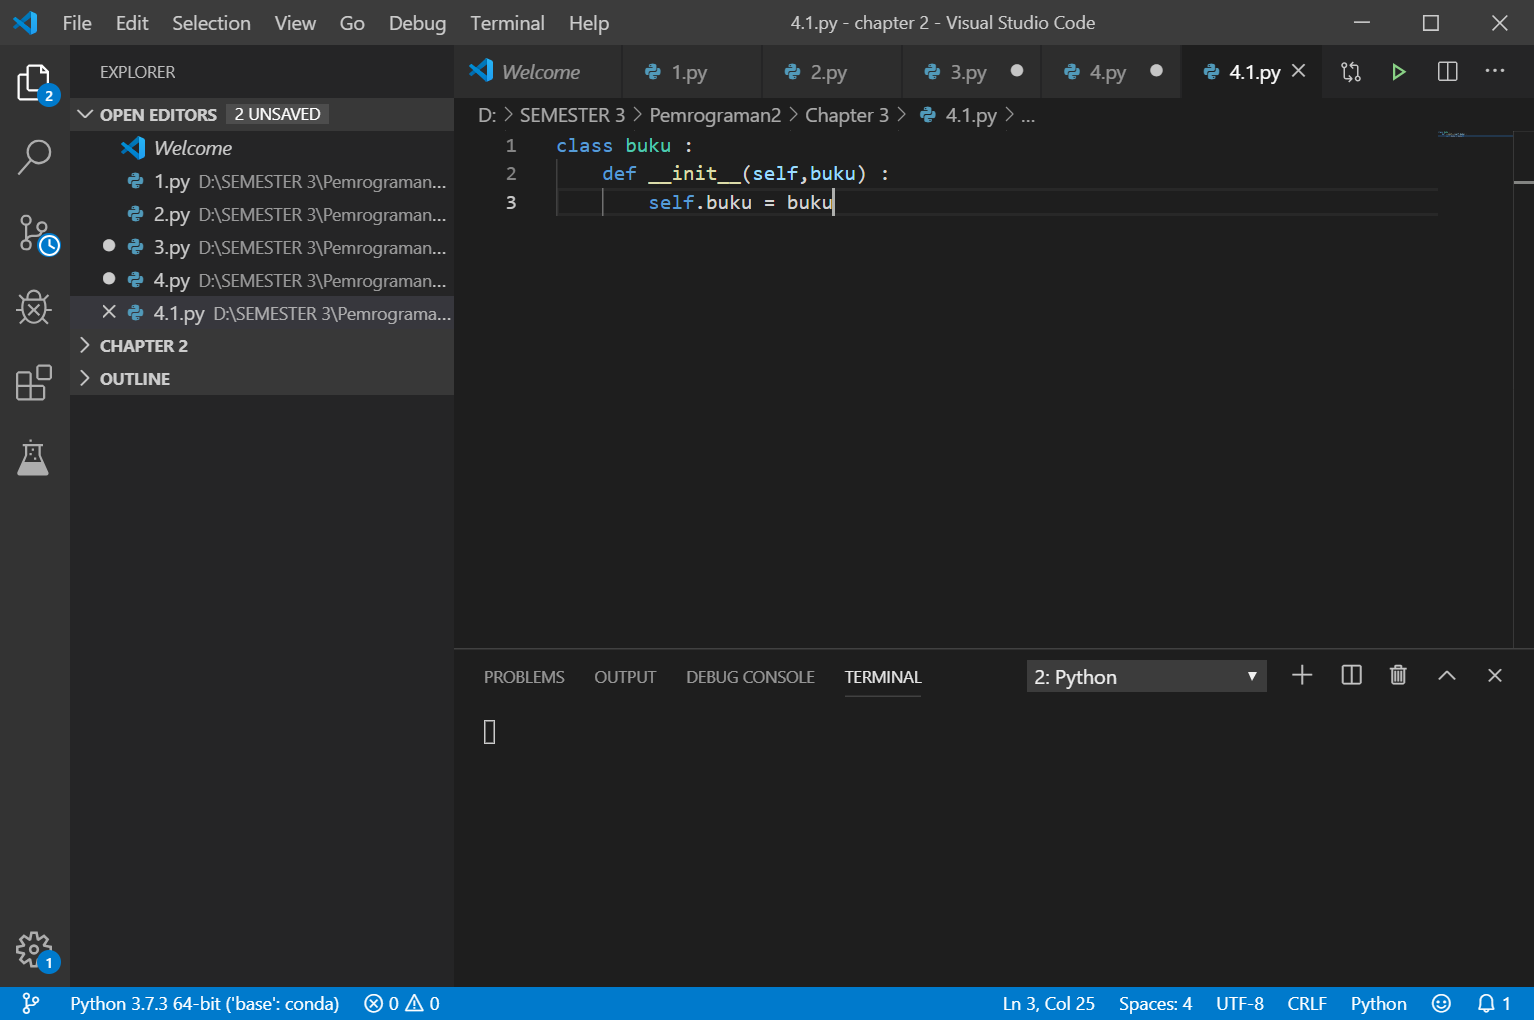
\includegraphics[width=.8\textwidth]{keterampilan/4.1.PNG}
\end{center}

\subsection{Method}
Method merupakan fungsi atau program yang ada dalam sebuah class.
\begin{center}
    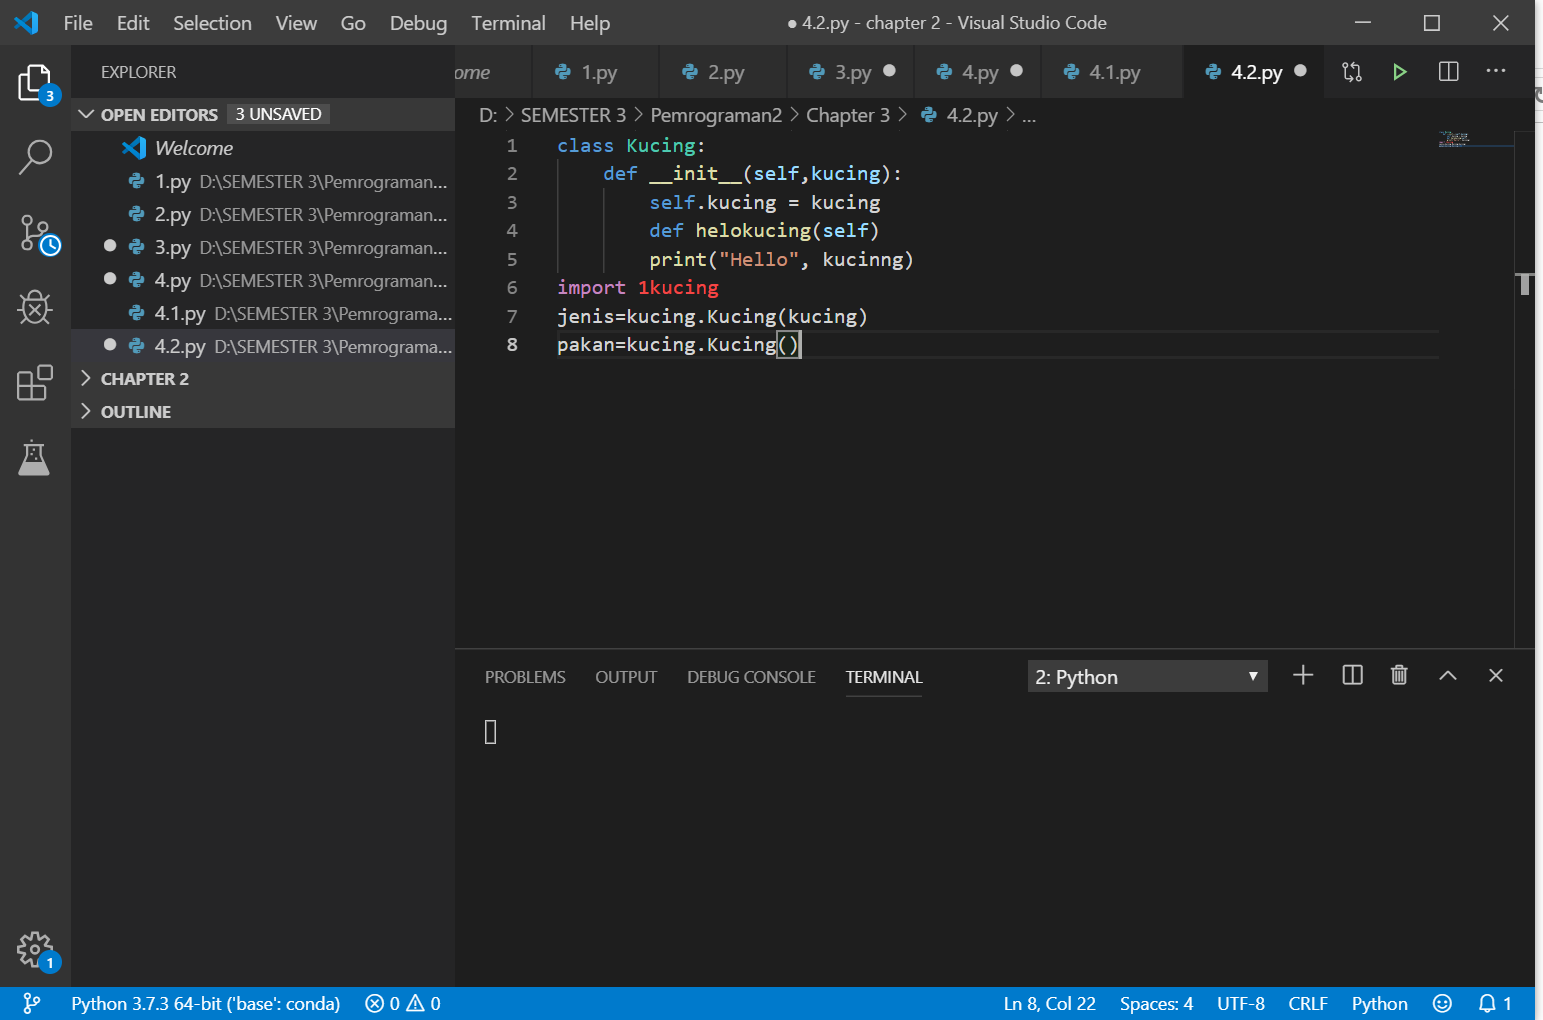
\includegraphics[width=.8\textwidth]{keterampilan/4.2.PNG}
\end{center}

\section{Penggunaan Library}
\begin{center}
    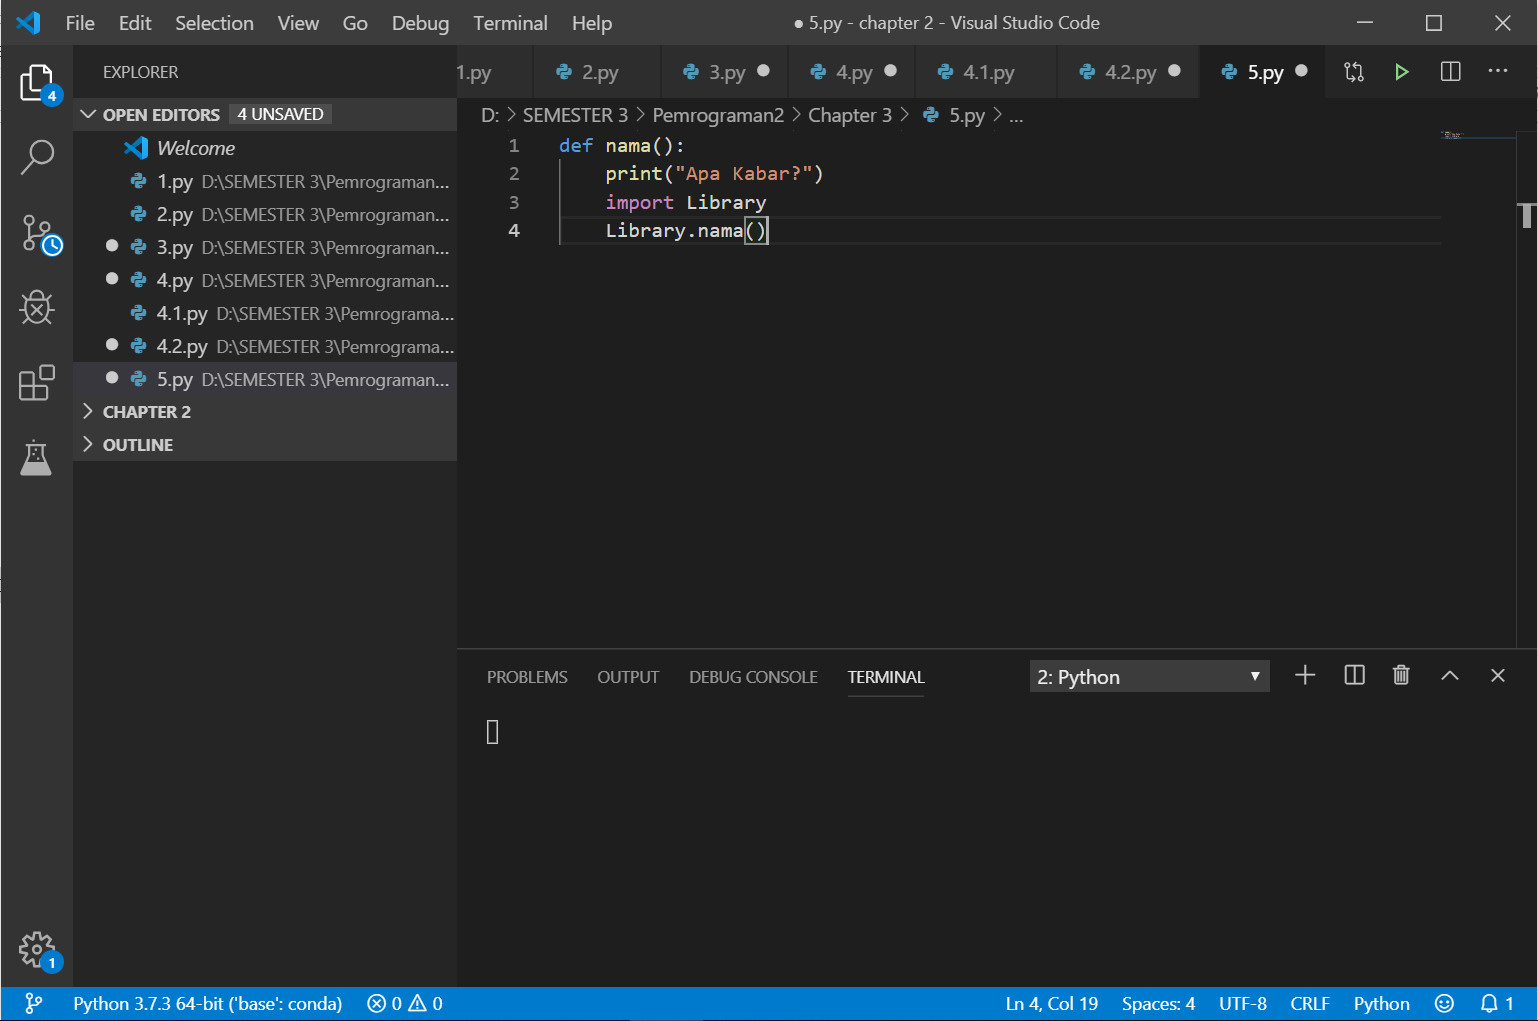
\includegraphics[width=.8\textwidth]{keterampilan/5.PNG}
\end{center}

\section{Pemakaian Package From Kalkulator Import penambahan}
\begin{center}
    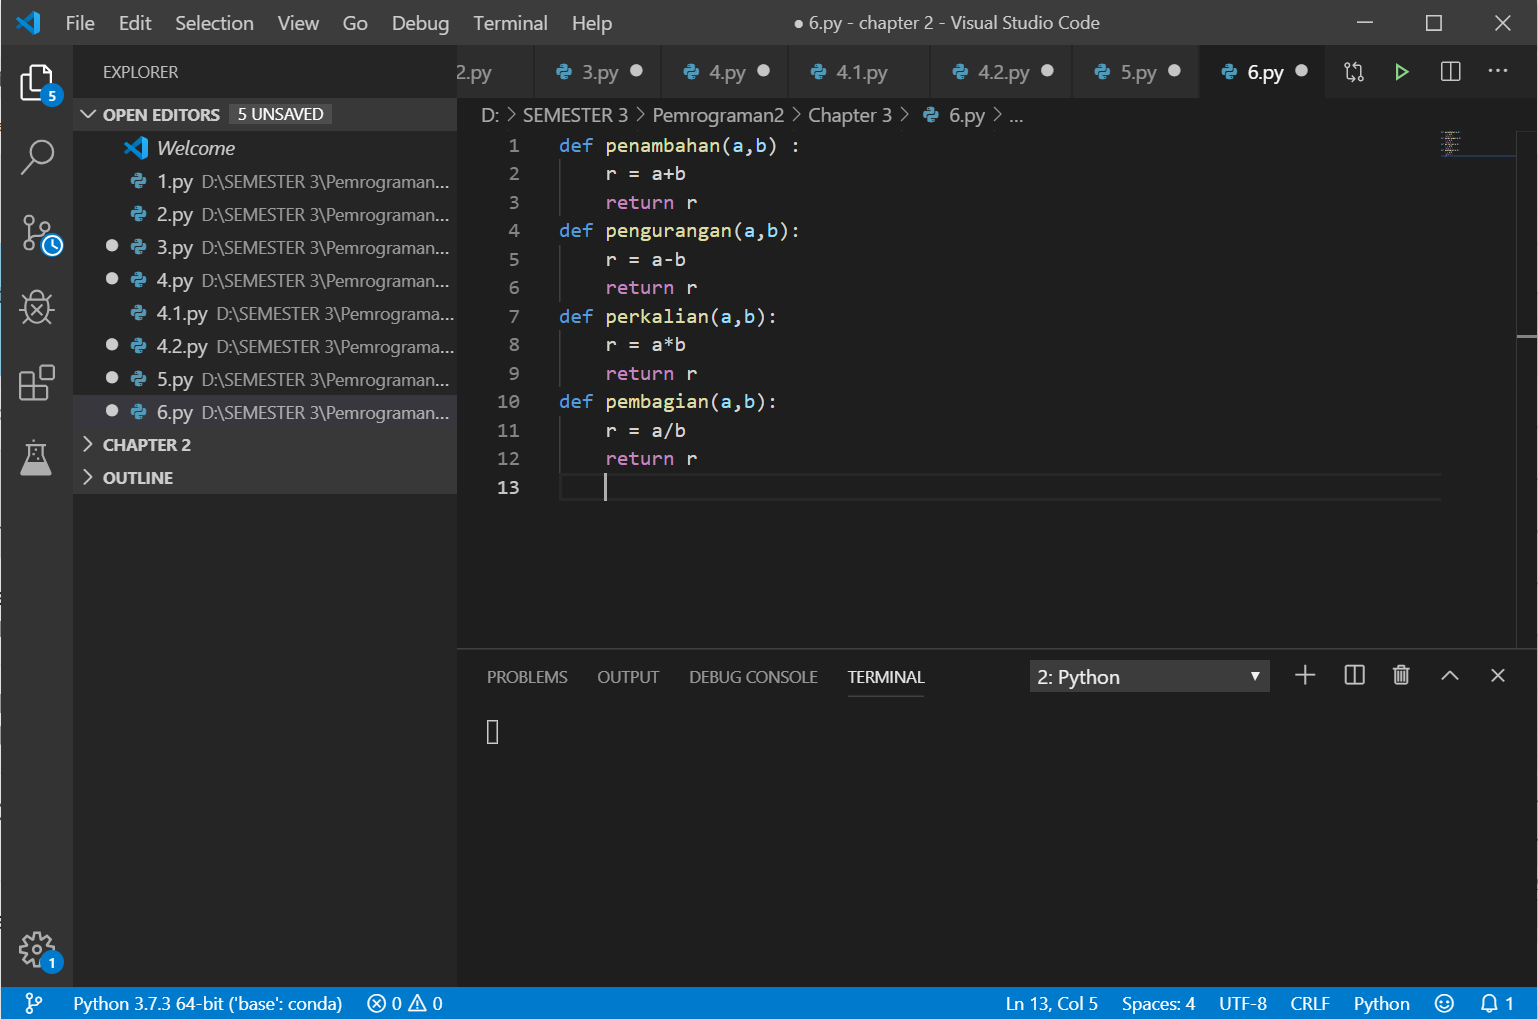
\includegraphics[width=.8\textwidth]{keterampilan/6.PNG}
    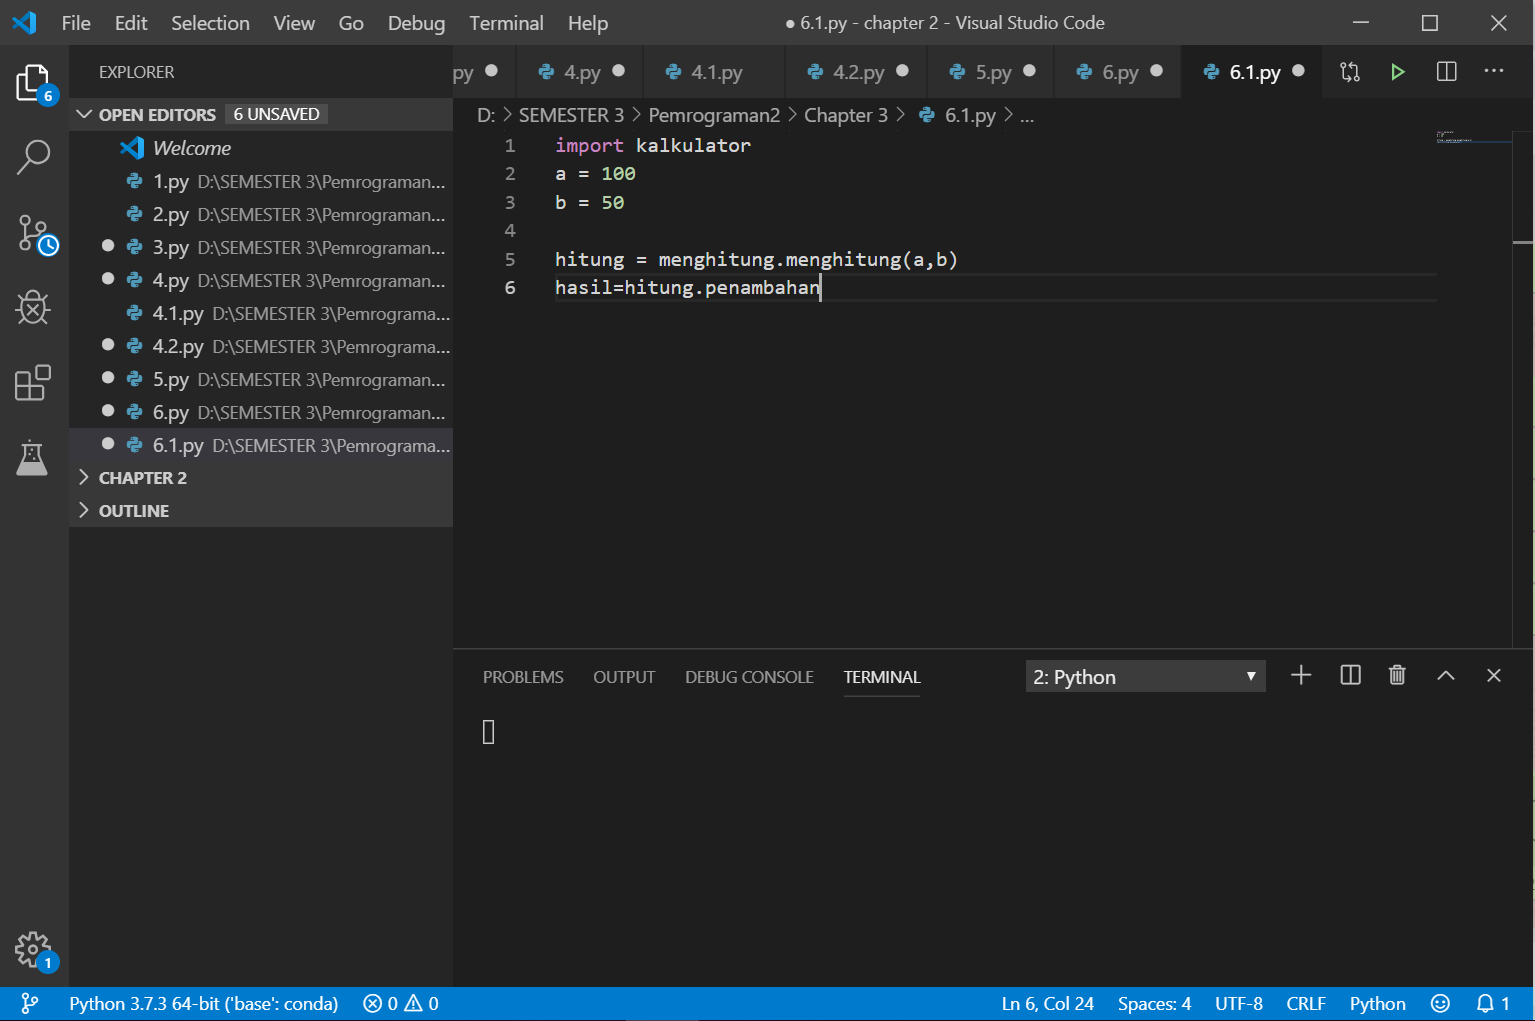
\includegraphics[width=.8\textwidth]{keterampilan/6.1.PNG}
\end{center}

\section{Pemanggilan Library dalam Sebuah Folder}
untuk memanggil sebuah library dalam sebuah folder yang pertama yang harus di panggil adalah nama foldernya terlebih dahulu, lalu import library
\begin{center}
    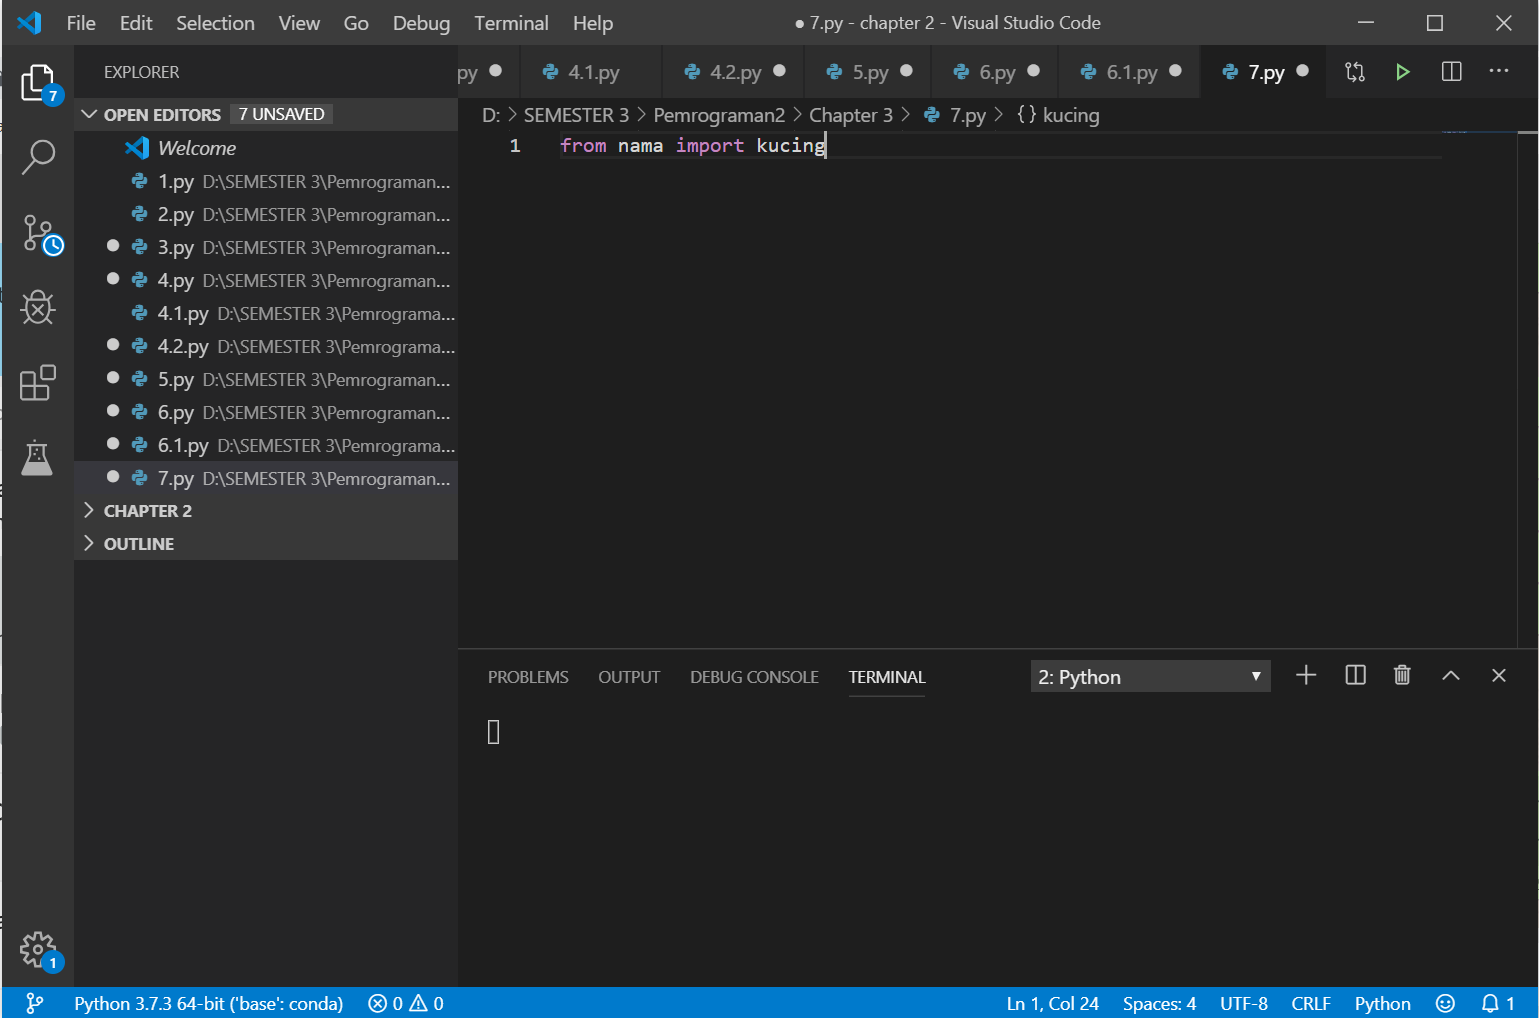
\includegraphics[width=.8\textwidth]{keterampilan/7.PNG}
\end{center}

\section{Pemanggilan Class dalam Sebuah Folder}
untuk memanggil sebuah class dalam sebuah folder yang pertama yang harus di panggil adalah nama foldernya terlebih dahulu, lalu import class

\begin{center}
    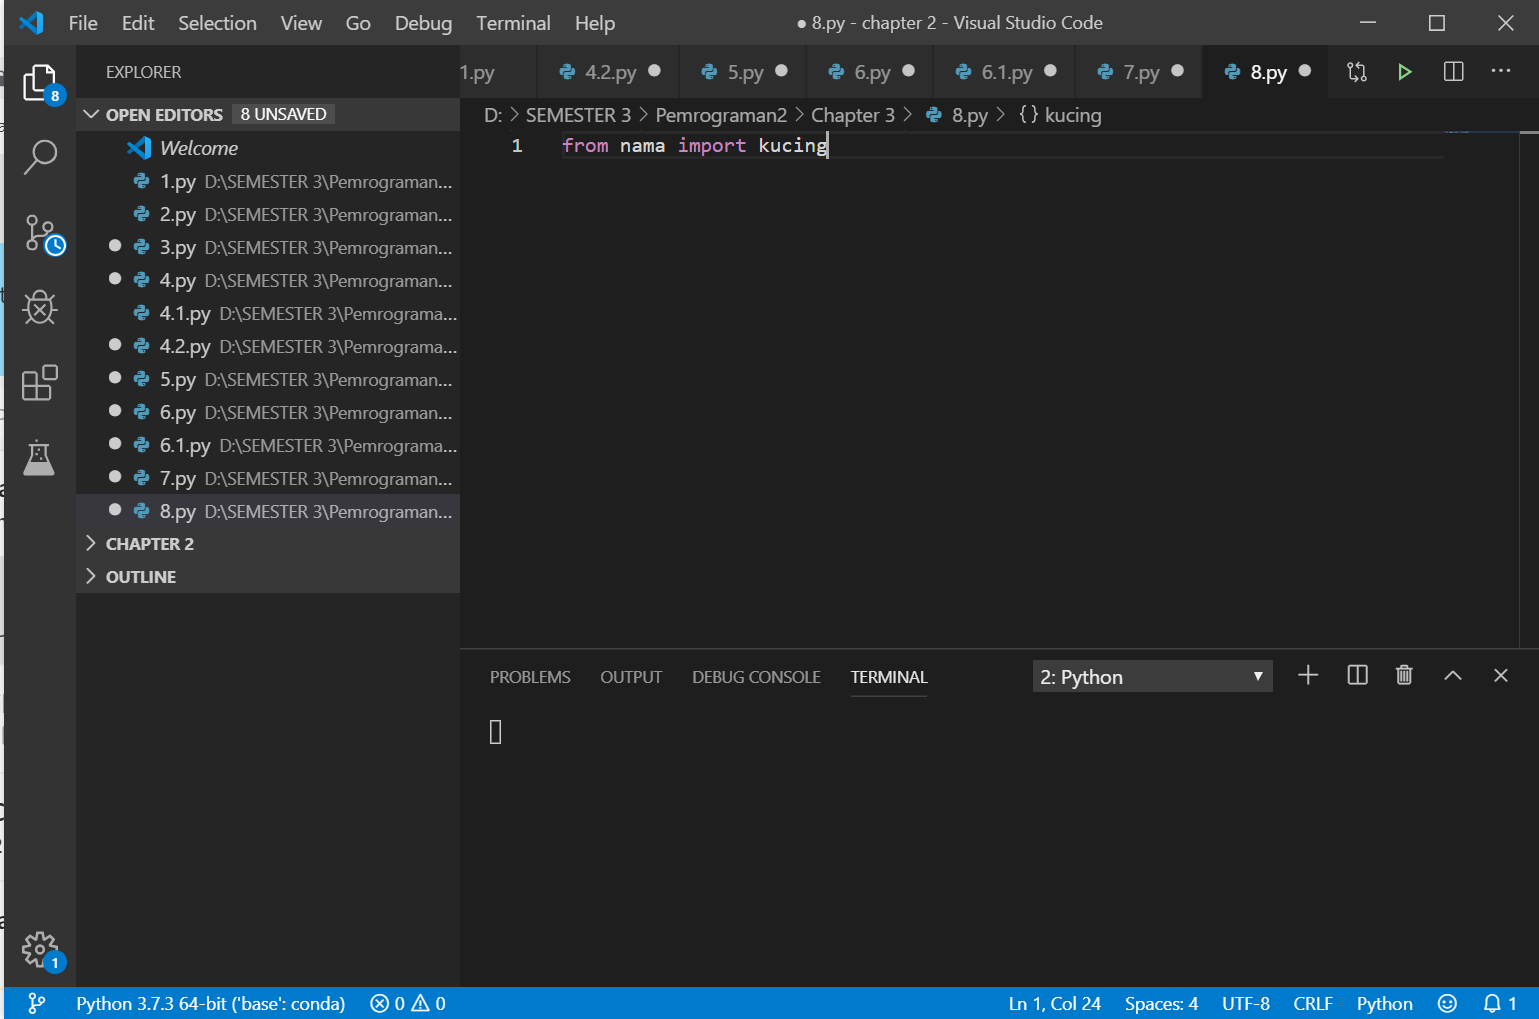
\includegraphics[width=.8\textwidth]{keterampilan/8.PNG}
\end{center}



\section{Keterampilan}
\begin{enumerate}
    \item Buatlah luaran huruf yang dirangkai dari tanda bintang, pagar atau plus dari
    NPM kita. Tanda bintang untuk NPM mod 3=0, tanda pagar untuk NPM mod
    3 =1, tanda plus untuk NPM mod3=2
\begin{center}
    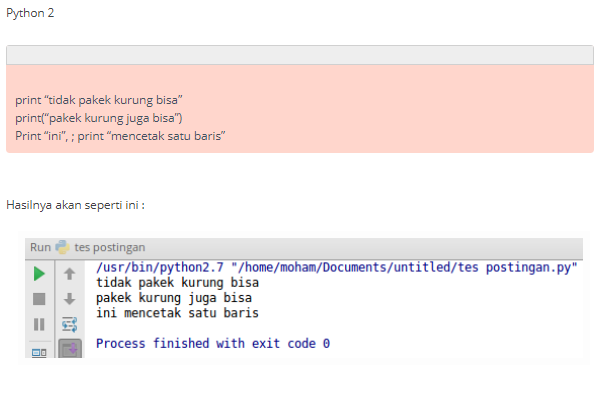
\includegraphics[width=.8\textwidth]{1.PNG}
\end{center}

    \item Buatlah program hello word dengan input NPM yang disimpan dalam sebuah
    variabel string bernama NPM dan output sebanyak dua dijit belakang NPM,
    contoh NPM : 113040087 maka akan ada output sebanyak 87 dengan tulisan ‘Hallo, 113040087 apa kabar?’ \\

    NPM=int(input("masukkan NPM :")) \\
    i=NPM%100 \\
    for i in range(i): \\
    print("hello",NPM,"apa kabar?")\\
\begin{center}
    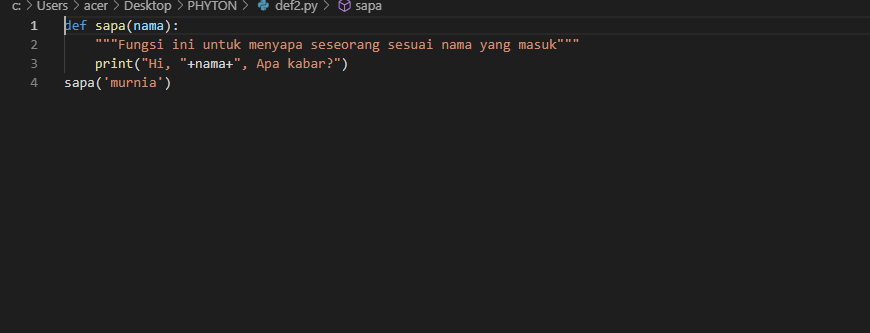
\includegraphics[width=.8\textwidth]{2.PNG}
\end{center}

\item Buatlah program hello word dengan input nama yang disimpan dalam sebuah variabel string bernama NPM dan beri luaran output berupa tiga karakter belakang dari NPM sebanyak penjumlahan tiga dijit tersebut, \\
NPM=input("Masukan Npm anda: ")\\
X =int (NPM[4])\\
Y =int (NPM[5])\\
Z =int (NPM[6])\\
hitung1 = X + Y + Z\\
hitung2 = X + Y + Z\\
while hitung1 > 0:\\
        print("Hallo, " , NPM[4:7], "Apa kabar ?")\\
        hitung1 = hitung1 -1 \\
print("...",str(hitung2),"kali(",str(X),"+",str(Y),"+"+str(Z),")...")\\
\begin{center}
    \includegraphics[width=.8\textwidth]{3.PNG}
\end{center}

\item Buatlah program hello word dengan input nama yang disimpan dalam sebuah variabel string bernama NPM dan beri luaran output berupa digit ketiga dari belakang dari variabel NPM,\\
NPM = input("Npm anda: ")\\
print("Hallo, ",NPM[4],"Apa kabar ?")\\
\begin{center}
    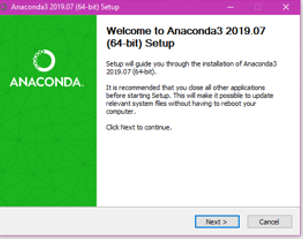
\includegraphics[width=.8\textwidth]{4.PNG}
\end{center}

\item (untuk soal no 5 dan selanjutnya wajib menggunakan perulangan dan kondisi) buat program dengan mengisi variabel alfabet dengan nomor npm satu persatu berurut.\\
i=0 \\
NPM = input("Npm anda: ")\\
while i <1:\\
    if len(NPM) <7:\\
        print("NPM anda kurang dari 7!")\\
        NPM = input("NPM anda: ")\\
    elif len(NPM) >7:\\
        print ("NPM lebih dari 7!")\\
        NPM = input ("NPM anda: ")\\
    else:\\
        i=1\\

A=NPM[0]\\
B=NPM[1]\\
C=NPM[2]\\
D=NPM[3]\\
E=NPM[4]\\
F=NPM[5]\\
G=NPM[6]\\

for this in A,B,C,D,E,F,G:\\
    print (this,end =" "),\\
\begin{center}
    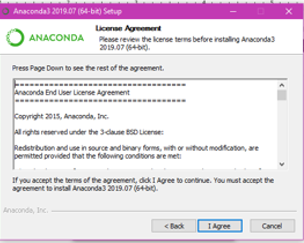
\includegraphics[width=.8\textwidth]{5.PNG}
\end{center}

\item Dari soal no 5, Lakukan penjumlahan dari seluruh variabel tersebut,\\
i=0\\
NPM = input("Npm anda: ")\\
while i <1:\\
    if len(NPM) <7:\\
        print("NPM anda kurang dari 7!")\\
        NPM = input("NPM anda: ")\\
    elif len(NPM) >7:\\
        print ("NPM lebih dari 7!")\\
        NPM = input ("NPM anda: ")\\
    else:\\
        i=1\\

A=NPM[0]\\
B=NPM[1]\\
C=NPM[2]\\
D=NPM[3]\\
E=NPM[4]\\
F=NPM[5]\\
G=NPM[6]\\

X=0\\

for this in A,B,C,D,E,F,G:\\
    X+=int(this)\\
print(X)\\
\begin{center}
    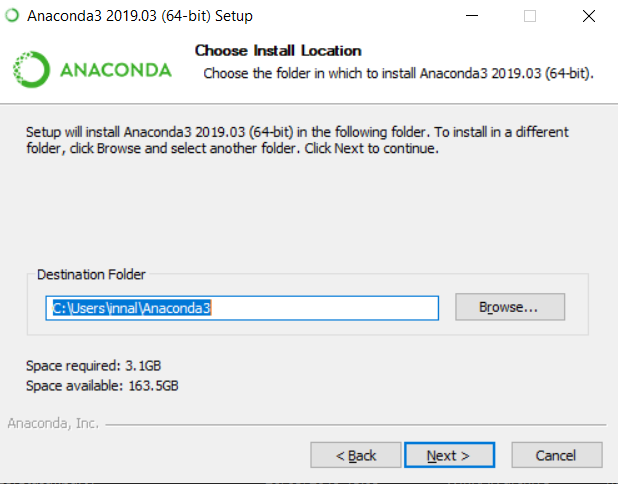
\includegraphics[width=.8\textwidth]{6.PNG}
\end{center}

\item Dari soal no 5, Lakukan perkalian dari seluruh variabel tersebut,\\
i=0\\
NPM = input("Npm anda: ")\\
while i <1:\\
    if len(NPM) <7:\\
        print("NPM anda kurang dari 7!")\\
        NPM = input("NPM anda: ")\\
    elif len(NPM) >7:\\
        print ("NPM lebih dari 7!")\\
        NPM = input ("NPM anda: ")\\
    else:\\
        i=1\\

A=NPM[0]\\
B=NPM[1]\\
C=NPM[2]\\
D=NPM[3]\\
E=NPM[4]\\
F=NPM[5]\\
G=NPM[6]\\

X=0\\

for this in A,B,C,D,E,F,G:\\
    X*=int(this)\\
print(X)\\
\begin{center}
    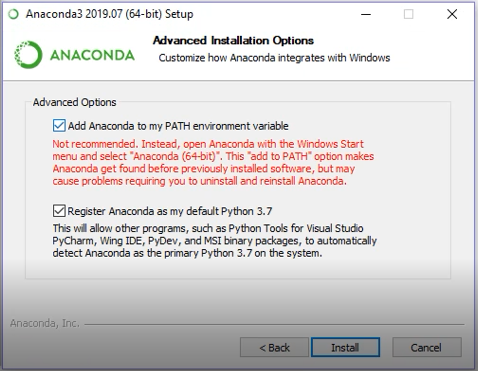
\includegraphics[width=.8\textwidth]{7.PNG}
\end{center}

\item Dari soal no 5, Lakukan print secara vertikal dari NPM anda menggunakan variabel diatas\\
i=0\\
NPM = input("Npm anda: ")\\
while i <1:\\
    if len(NPM) <7:\\
        print("NPM anda kurang dari 7!")\\
        NPM = input("NPM anda: ")\\
    elif len(NPM) >7:\\
        print ("NPM lebih dari 7!")\\
        NPM = input ("NPM anda: ")\\
    else:\\
        i=1\\

A=NPM[0]\\
B=NPM[1]\\
C=NPM[2]\\
D=NPM[3]\\
E=NPM[4]\\
F=NPM[5]\\
G=NPM[6]\\

X=0\\

for this in A,B,C,D,E,F,G:\\
    print(this)\\
\begin{center}
    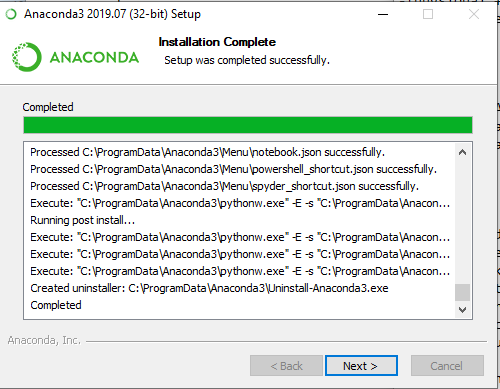
\includegraphics[width=.8\textwidth]{8.PNG}
\end{center}

\item Dari soal no 5, Lakukan print NPM anda tapi hanya dijit genap saja.\\
i=0\\
NPM = input("Npm anda: ")\\
while i <1:\\
    if len(NPM) <7:\\
        print("NPM anda kurang dari 7!")\\
        NPM = input("NPM anda: ")\\
    elif len(NPM) >7:\\
        print ("NPM lebih dari 7!")\\
        NPM = input ("NPM anda: ")\\
    else:\\
        i=1\\

A=NPM[0]\\
B=NPM[1]\\
C=NPM[2]\\
D=NPM[3]\\
E=NPM[4]\\
F=NPM[5]\\
G=NPM[6]\\

X=1\\

for this in A,B,C,D,E,F,G:\\
    
    if int (this)%2==0:\\
        if int(this)==0:\\
            this==""\\
        print(this,end=" ")\\
\begin{center}
    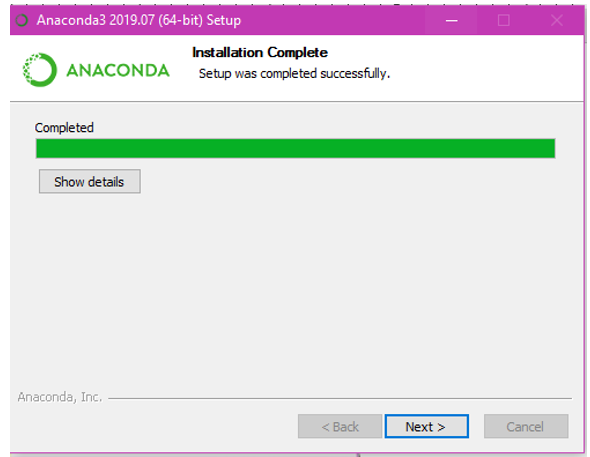
\includegraphics[width=.8\textwidth]{9.PNG}
\end{center}

\item Dari soal no 5, Lakukan print NPM anda tapi hanya dijit ganjil saja.\\
i=0\\
NPM = input("Npm anda: ")\\
while i <1:\\
    if len(NPM) <7:\\
        print("NPM anda kurang dari 7!")\\
        NPM = input("NPM anda: ")\\
    elif len(NPM) >7:\\
        print ("NPM lebih dari 7!")\\
        NPM = input ("NPM anda: ")\\
    else:\\
        i=1\\

A=NPM[0]\\
B=NPM[1]\\
C=NPM[2]\\
D=NPM[3]\\
E=NPM[4]\\
F=NPM[5]\\
G=NPM[6]\\

X=1\\

for this in A,B,C,D,E,F,G:\\
    
    if int (this)%2==0:\\
        if int(this)==0:\\
            this==""\\
        print(this,end=" ")\\
\begin{center}
    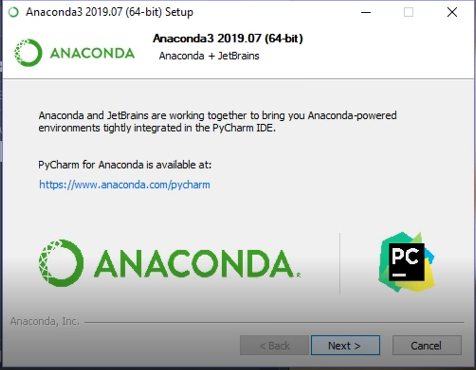
\includegraphics[width=.8\textwidth]{10.PNG}
\end{center}

\item
\begin{center}
    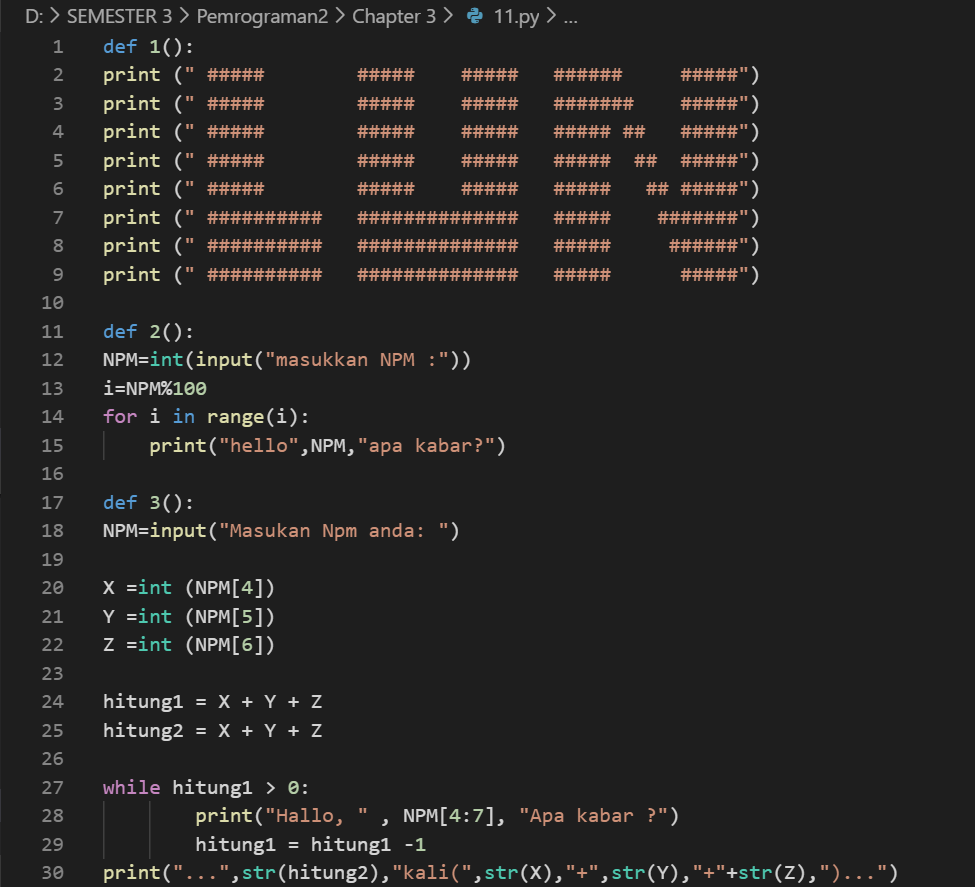
\includegraphics[width=.8\textwidth]{11-1.PNG}
    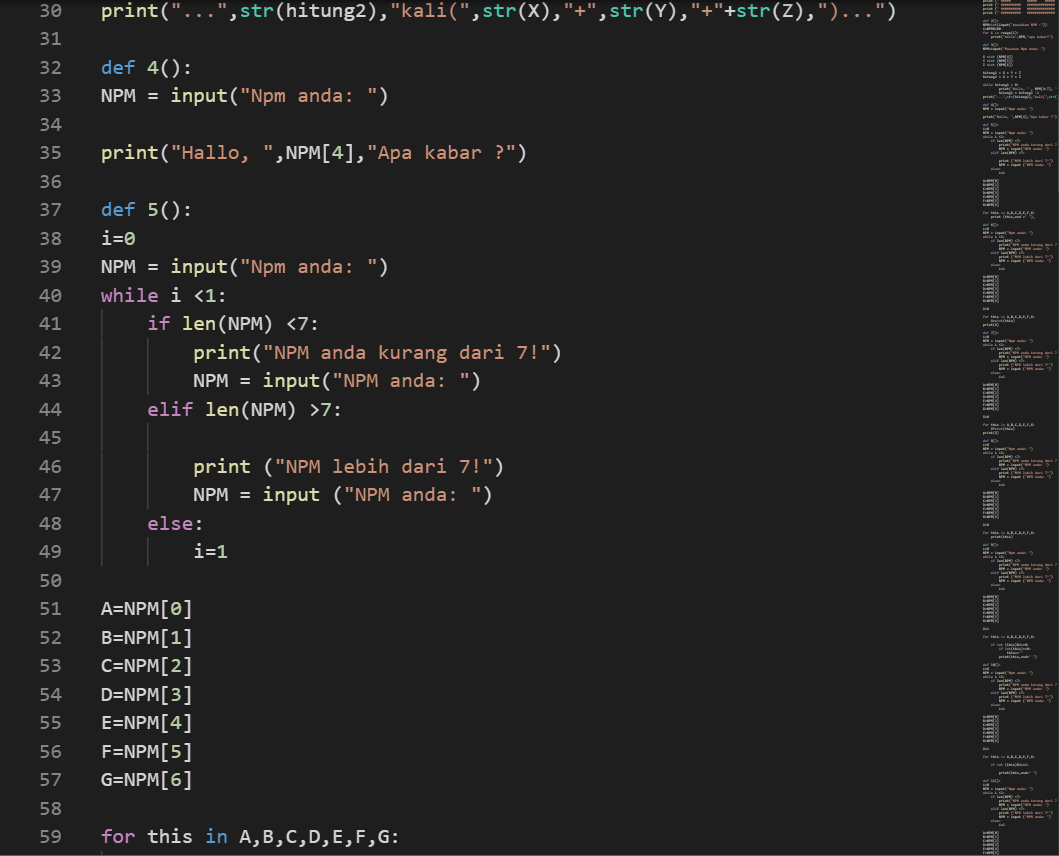
\includegraphics[width=.8\textwidth]{11-2.PNG}
    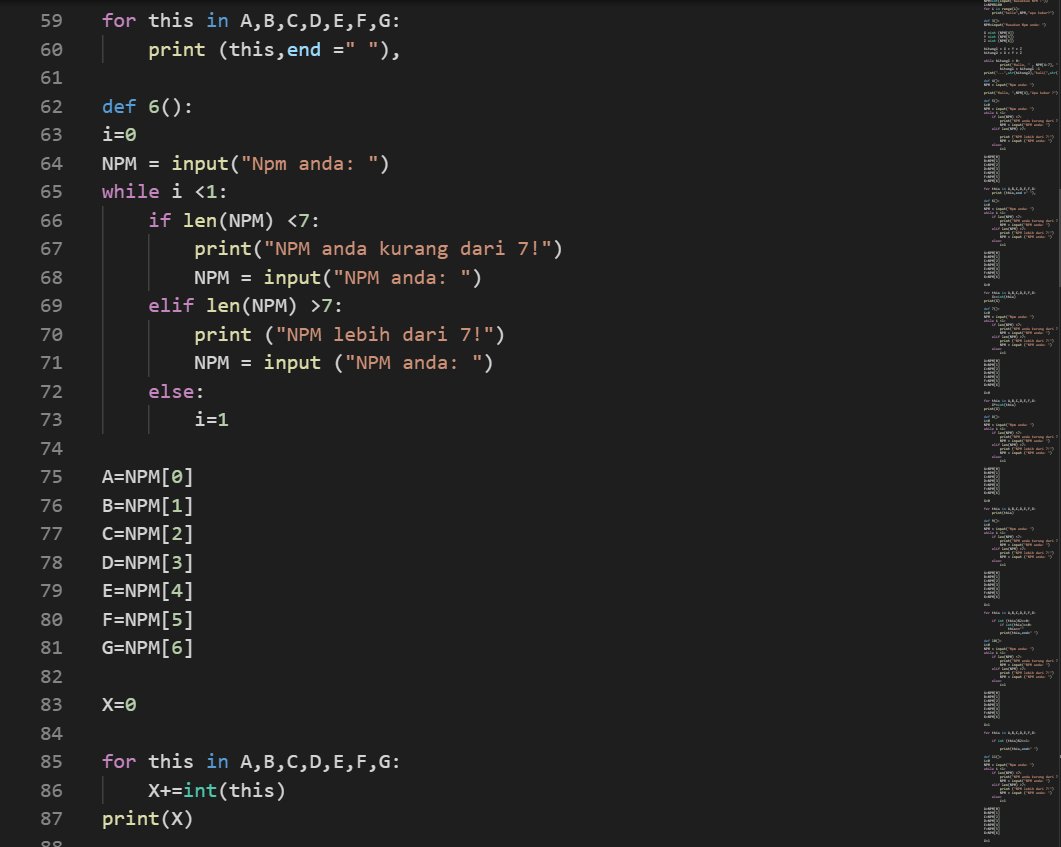
\includegraphics[width=.8\textwidth]{11-3.PNG}
    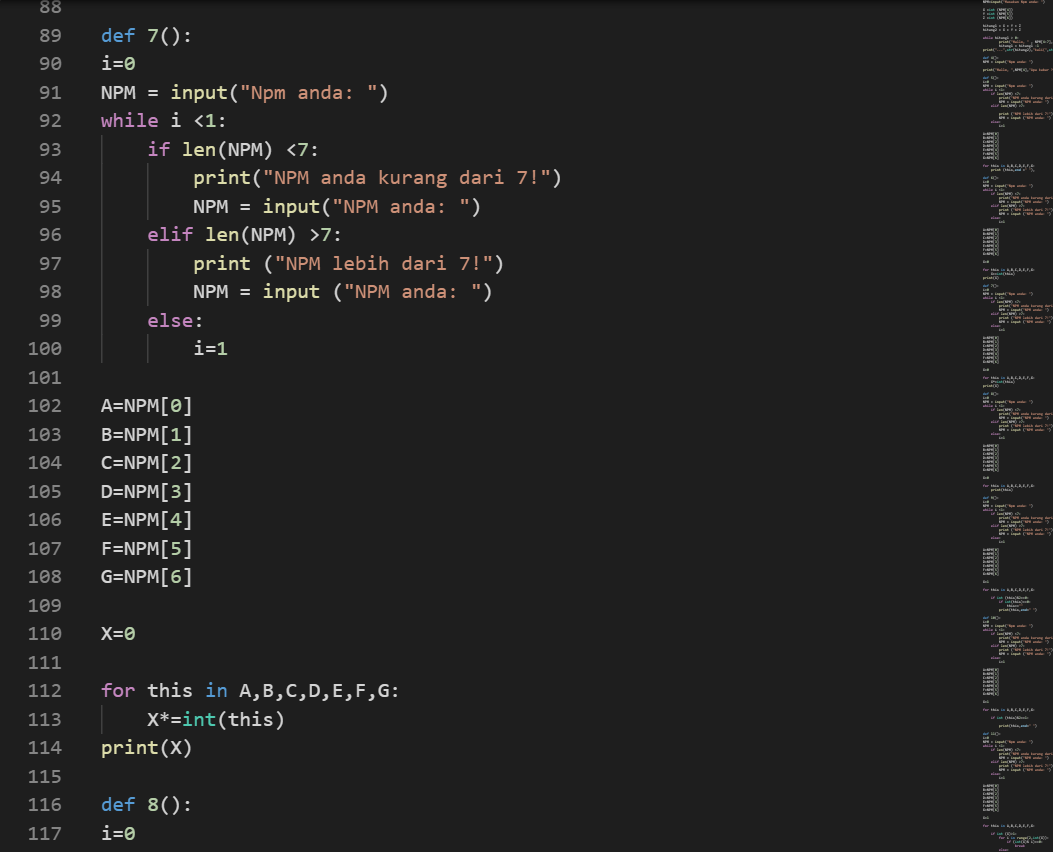
\includegraphics[width=.8\textwidth]{11-4.PNG}
    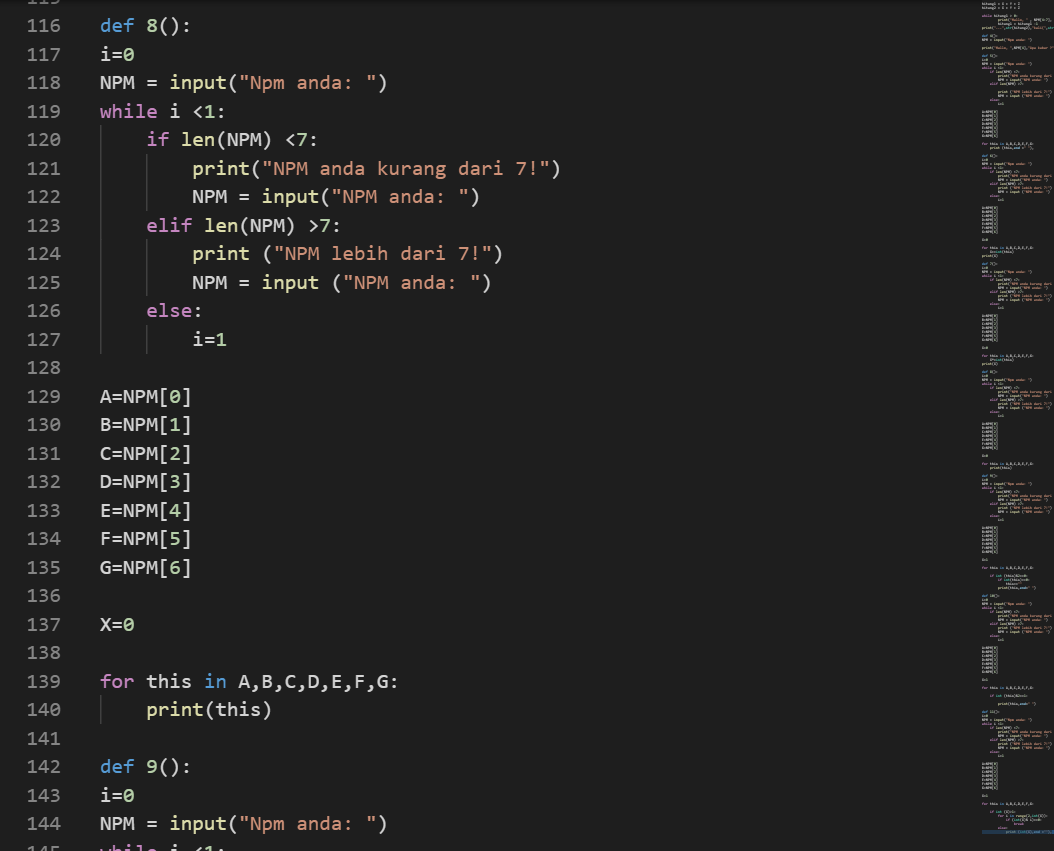
\includegraphics[width=.8\textwidth]{11-5.PNG}
    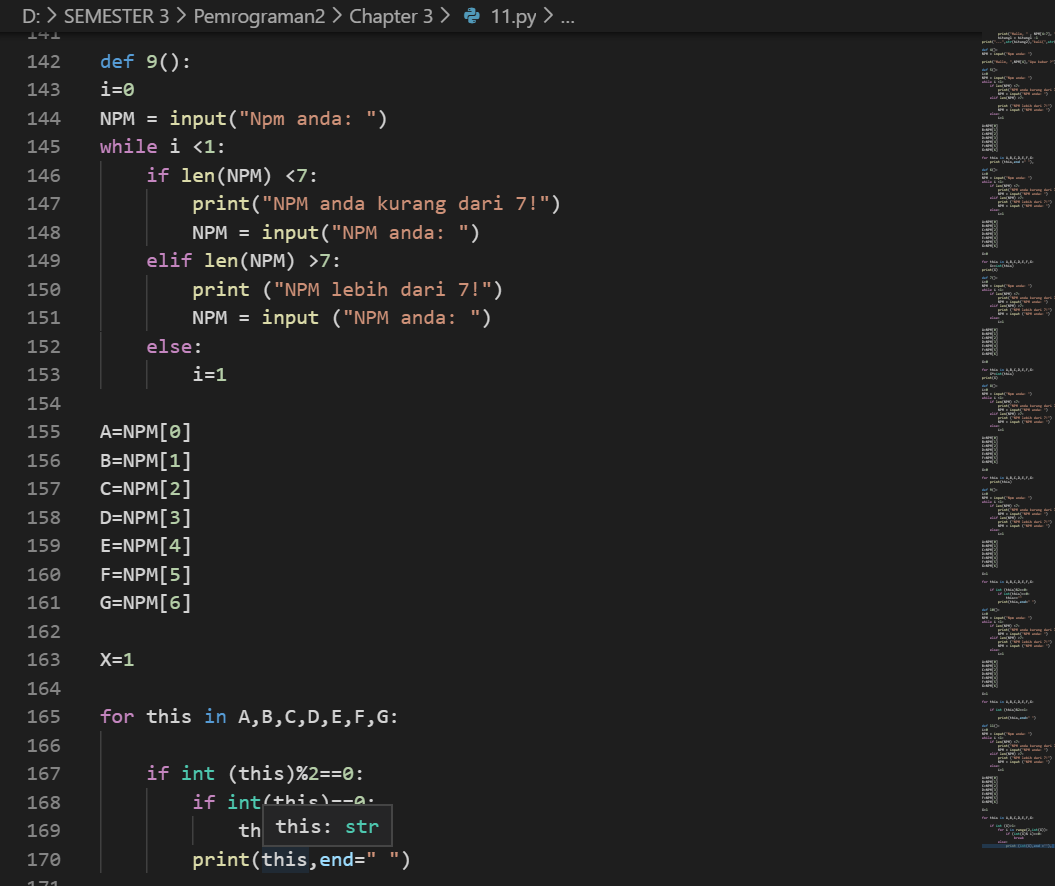
\includegraphics[width=.8\textwidth]{11-6.PNG}
    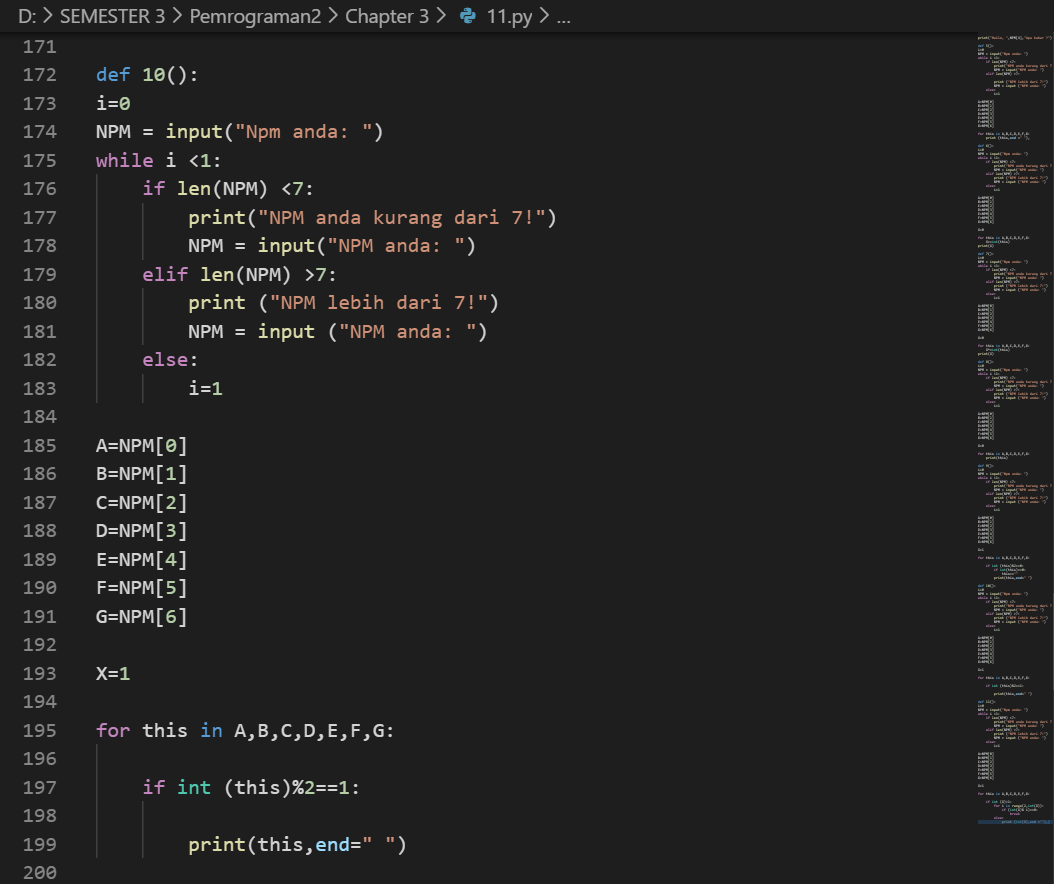
\includegraphics[width=.8\textwidth]{11-7.PNG}
    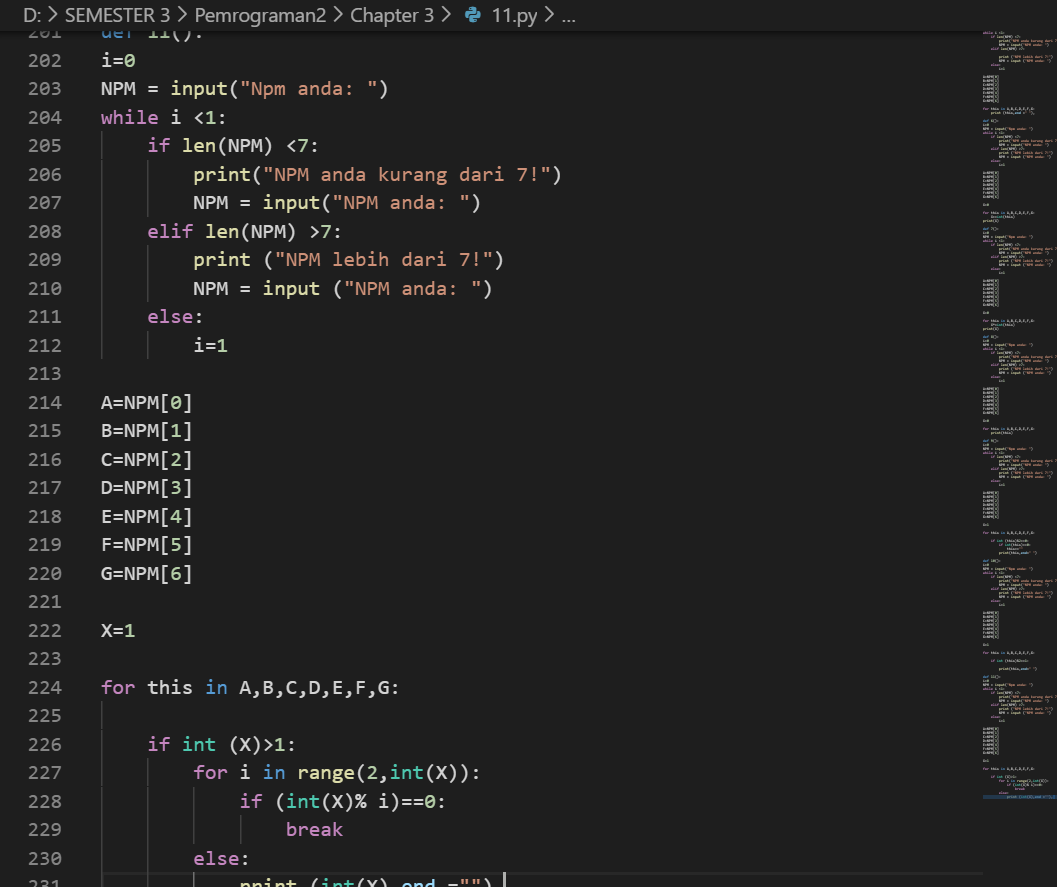
\includegraphics[width=.8\textwidth]{11-8.PNG}
           
\end{center}

\item 
\begin{center}
    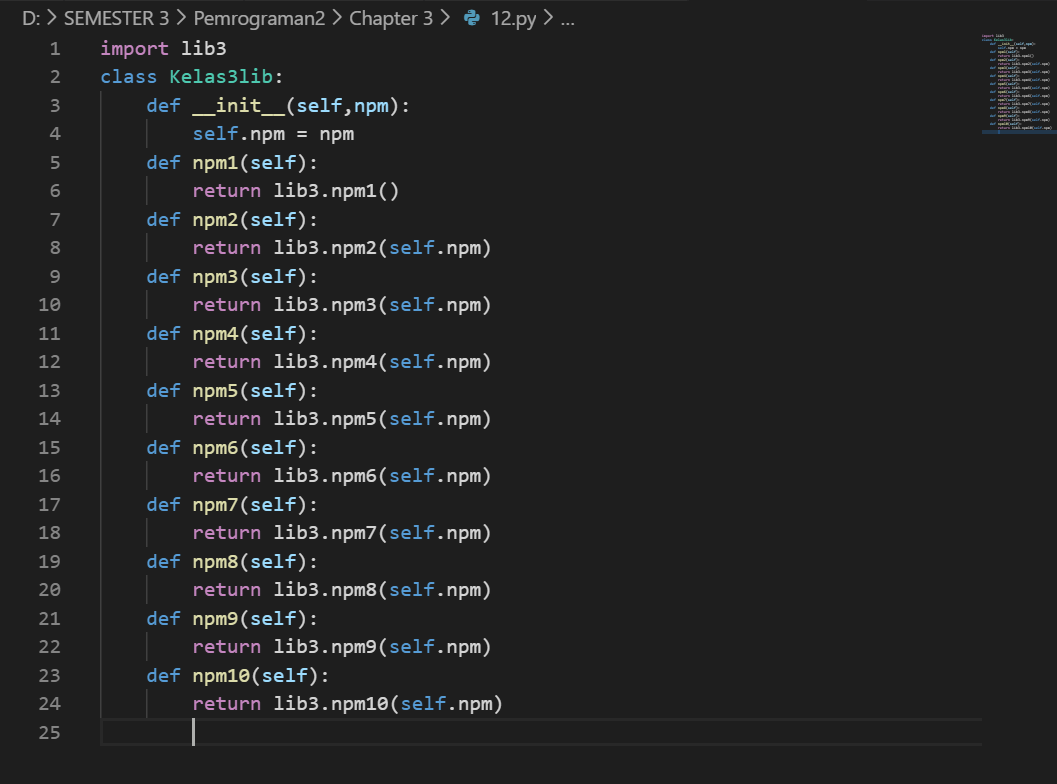
\includegraphics[width=.8\textwidth]{12.PNG}
    
    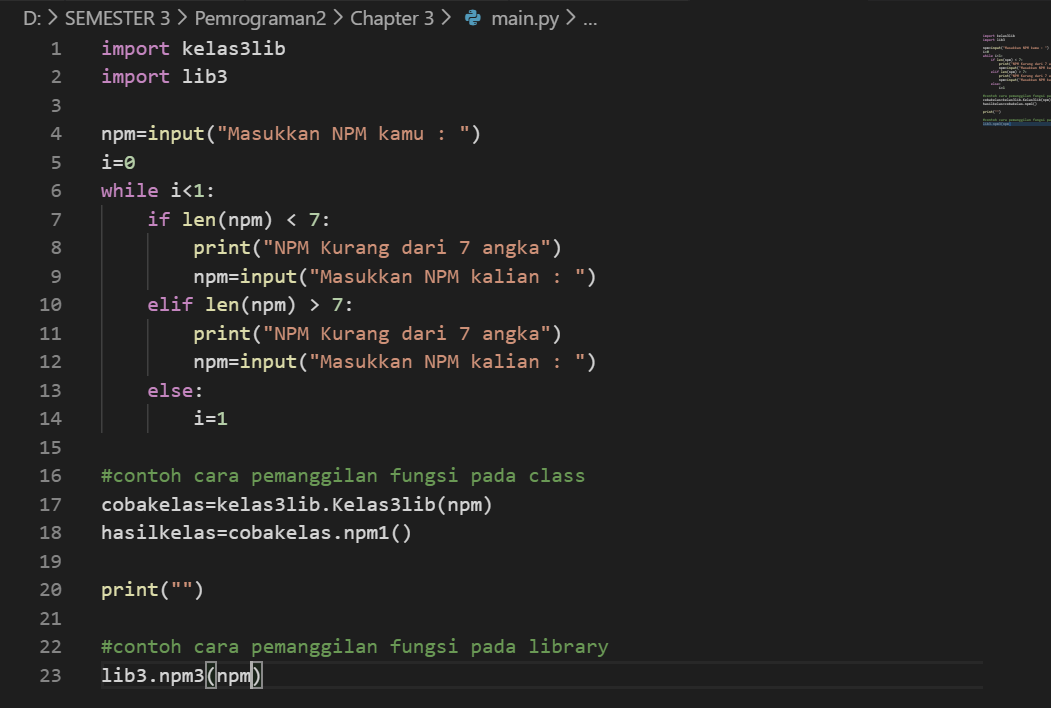
\includegraphics[width=.8\textwidth]{main.PNG}

\end{center}

\section{Keterampilan Penanganan Error}
\begin{center}
    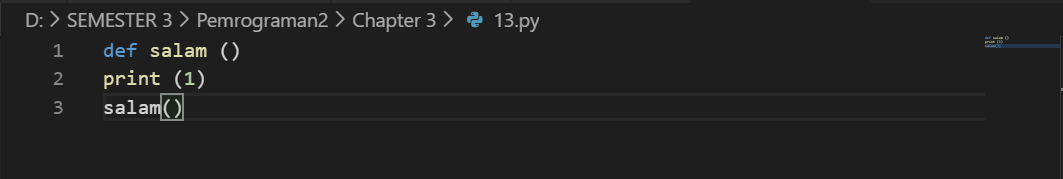
\includegraphics[width=.8\textwidth]{13.PNG}
    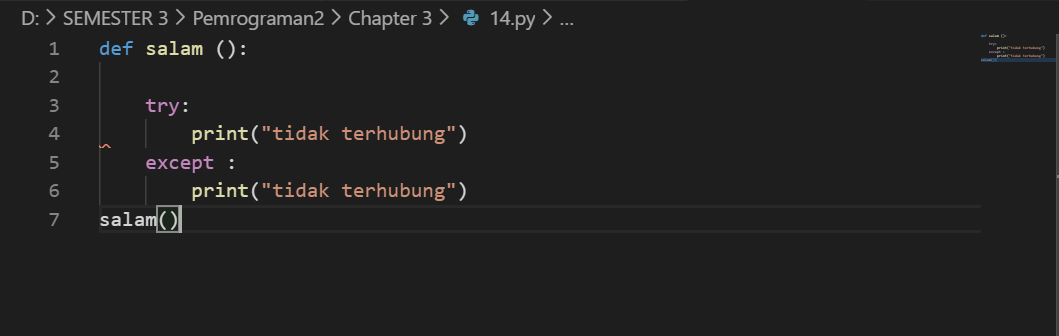
\includegraphics[width=.8\textwidth]{14.PNG}
\end{center}


\end{enumerate}

\end{document}

